\section{Udgangstrinsklasser}
\label{klasser}
En HiFi-forstærkers udgangstrin kan designes på forskellige måder alt efter hvilken funktionalitet der ønskes. De forskellige designs er opdelt i klasser. Klasserne er bestemt ud fra trinnets karakteristika og ikke ud fra en bestemt opkobling af kredsløbet. Karakteristika, som er vigtige at tage i betragtning, for udgangstrinnet i en HiFi-forstærker er nyttevirkning, strømvinkel og forvrængning. Nyttevirkningen er givet ved hvor stor en procentdel af den totale effekt leveret af forsyning, der bliver afsat i belastningen, i dette tilfælde højtaleren.
I dette afsnit vil der blive gjort rede for klasse A, B og AB samt forklaret hvilke fordele og ulemper der er med dem. Redegørelsen vil tage udgangspunkt i ovenstående karakteristika samt demonstrere en mulig opbygning af trinnet.
Der vil, på baggrund af dette afsnit, blive valgt en endelig udgangstrinsklasse til dette projekts HiFi-forstærker hvilket vil blive et krav i kravspecifikationen.

\subsection{Klasse A}

Et klasse A udgangstrin har en strømkarakteristik på udgangen, som vist på figur \ref{fig:klassea} med en sinustone, som indgangssignal. 

\begin{figure}[ht]
\begin{minipage}[b]{0.5\linewidth}
\centering
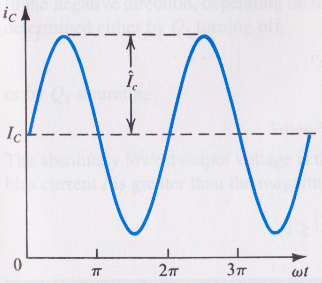
\includegraphics[scale=.35]{valg_af_loesning/klasser/klassea.png}
\caption{Klasse A $i_c (Q1)$ karakteristik\cite{sedra-smith}}
\label{fig:klassea}
\end{minipage}
\hspace{0.5cm}
\begin{minipage}[b]{0.5\linewidth}
\centering
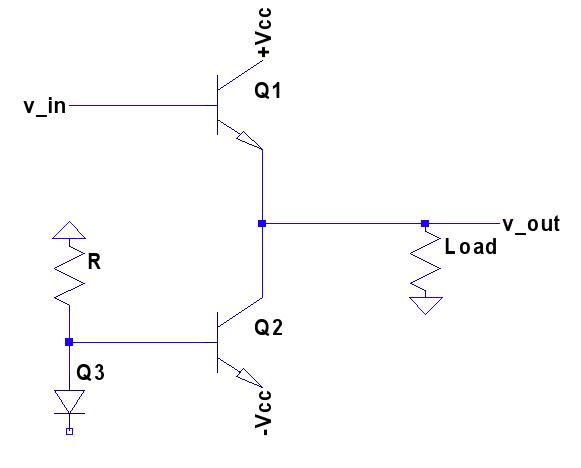
\includegraphics[scale=.35]{valg_af_loesning/klasser/classa.png}
\caption{Eksempel på klasse A udgangstrinskredsløb\cite{sedra-smith}}
\label{fig:classa}
\end{minipage}
\end{figure}


Et klasse A udgangstrin kan opbygges af to NPN transistorer, Q1 og Q2, i en emitterfølgerkobling, som vist på figur \ref{fig:classa}. En konstant strøm løber gennem Q2, da $v_{\mathrm{BE2}}$ er konstant. Inputsignalet kommer ind på Q1's base og styrer således strømmen der kan løbe gennem Q1 og belastningsmodstanden. 

Et klasse A udgangstrin har en strømvinkel på udgangstransistoren på 360°. Dette viser sig nyttigt i det at indgangssignalet er repræsenteret på udgangen i sin komplette form, hvilket giver en lav forvrængning.
I et klasse A udgangstrin løber altid en konstant strøm gennem Q2, hvis kredsløbet på figur \ref{fig:classa} benyttes. Dette gør at den maksimale teoretiske nyttevirkning kun er 25\%. \cite{sedra-smith}%\fixme{kilde: til sedra smith}

\subsection{Klasse B}

Et klasse B udgangstrin har en strømkarakteristik på udgangen, som vist på figur \ref{fig:klasseb} med en sinustone, som indgangssignal. 

\begin{figure}[ht]
\begin{minipage}[b]{0.5\linewidth}
\centering
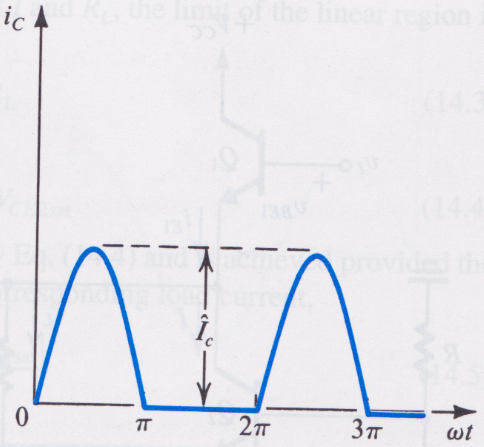
\includegraphics[scale=.35]{valg_af_loesning/klasser/klasseb.png}
\caption{Klasse B $i_c (Q1)$ karakteristik\cite{sedra-smith}}
\label{fig:klasseb}
\end{minipage}
\hspace{0.5cm}
\begin{minipage}[b]{0.5\linewidth}
\centering
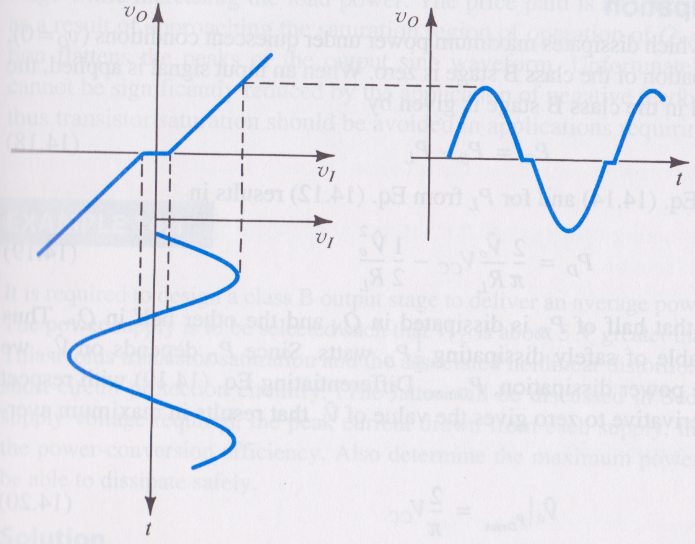
\includegraphics[scale=.25]{valg_af_loesning/klasser/klassebproblem.png}
\caption{Eksempel på klasse B udgangstrin med crossoverdistortion\cite{sedra-smith}}
\label{fig:classbproblem}
\end{minipage}
\end{figure}


I eksemplet på figur \ref{fig:classb} er klasse B udgangstrinnet opbygget af to transistorer, en NPN (Q1) og en PNP (Q2). Når input spændingen overstiger ca. 0,6 V vil Q1 begynde at lede strøm til belastningsmodstanden mens Q2 er lukket. Kommer input spændingen under -0,6 V vil Q2 lede, men da Q2 er en PNP vil den trække strøm mod -Vcc hvormed der trækkes strøm fra belastningsmodstanden. Når Q2 leder er Q1 lukket. 

Et klasse B udgangstrin overfører kun en halv periode af indgangssignalet til udgangen, altså er strømvinklen 180°. For at kunne gengive et udgangssignal similært til indgangssignalet er det derfor nødvendigt at sammensætte to klasse B udgangstrin således at det ene tager sig af den positive halvperiode og den anden den negative. Dette giver anledning til et fænomen kaldet crossoverdistortion. Dette fænomen optræder i dette tilfælde i overgangen fra den positive halvperiode til den negative og skyldes diodekarakteristikken i transistorernes base-emitter overgang. Crossoverdistortion for et klasse B udgangstrin er illustreret på figur \ref{fig:classbproblem}.
Et klasse B udgangstrin har en maksimal nyttevirkning på 78,5 \%. \cite{sedra-smith}%\fixme{kilde: til sedra smith}

\begin{figure}[h]
\centering
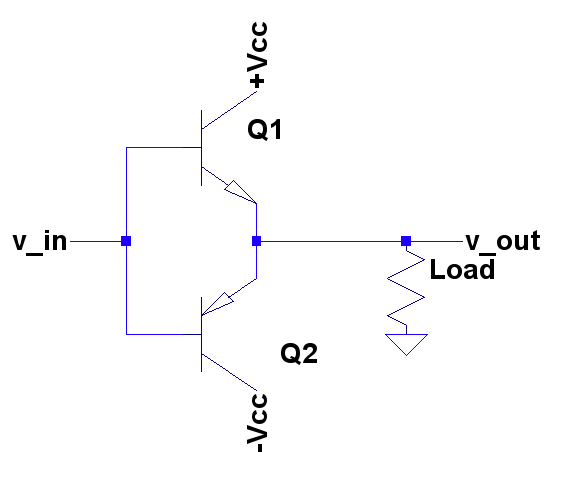
\includegraphics[scale=.35]{valg_af_loesning/klasser/classb.png}
\caption{Klasse B forstærker kredsløb\cite{sedra-smith}}
\label{fig:classb}
\end{figure}

\subsection{Klasse AB}
\label{klasse_ab}

Et klasse AB udgangstrin har en strømkarakteristik på udgangen, som vist på figur \ref{fig:klasseab} med en sinustone, som indgangssignal. 

\begin{figure}[ht]
\begin{minipage}[b]{0.5\linewidth}
\centering
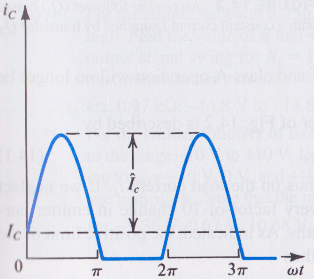
\includegraphics[scale=.35]{valg_af_loesning/klasser/klasseab.png}
\caption{Klasse AB $i_c$ karakteristik\cite{sedra-smith}}
\label{fig:klasseab}
\end{minipage}
\hspace{0.5cm}
\begin{minipage}[b]{0.5\linewidth}
\centering
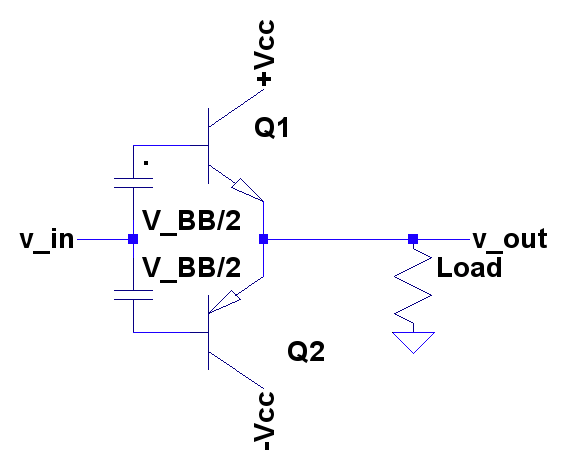
\includegraphics[scale=.35]{valg_af_loesning/klasser/classab.png}
\caption{Klasse AB forstærker kredsløb\cite{sedra-smith}}
\label{fig:classab}
\end{minipage}
\end{figure}


Der tages i eksemplet på et klasse AB udgangstrin på figur \ref{fig:classab} udgangspunkt i klasse B udgangstrinnet på figur \ref{fig:classb}, med den forskel at potentialet på Q1 og Q2's base er hævet til saturationspændingen når signalspændningen er 0 V. Det er denne forskel, som eleminerer crossoverdistortion.

Dette trin har en strømvinkel på mellem 180° og 360°. Dette bevirker at, hvis der bruges samme teknik, som ved et klasse B udgangstrin til at få en hel sinusperiode på udgangen, vil de to signaler overlappe i overgangsperioden. Dette medvirker til at crossoverdistortion, som forklaret for klasse B udgangstrinnet, elimineres. Dermed bliver forvrængningen for et klasse AB udgangstrin mindre end for et klasse B.
Et klasse AB udgangstrin har en nyttevirkning som ligger mellem den for et klasse A og et klasse B.

Et klasse AB udgangstrin har ikke et klasse A's lave nyttevirkning eller et klasse B's crossoverdistortion og er på baggrund af dette blevet valgt, som det udgangstrin der vil blive arbejdet videre på.